\documentclass[aspectratio=169]{beamer}
\usetheme{simple}

\RequirePackage[l2tabu, orthodox]{nag}


% \usepackage[left=1.in, right=1.in, top=1.25in, bottom=1.25in]{geometry}

% FONTS
%\usepackage[T1]{fontenc}

% Replace default Latin Modern typewriter with its proportional counterpart
% http://www.tug.dk/FontCatalogue/lmoderntypewriterprop/
%\renewcommand*\ttdefault{lmvtt}


%%% OPTION 1 - Fourier Math + New Century Schoolbook + ParaType Sans

% % Import Fourier Math (this imposes its own New Century Schoolbook type)
% % http://www.ctan.org/tex-archive/fonts/fouriernc/
%\usepackage{fouriernc}
%\usepackage{amsmath}
% % Replace with TeX Gyre Schola version of New Century Schoolbook (must scale!)
% % http://www.tug.dk/FontCatalogue/tgschola/
%\usepackage[scale=0.92]{tgschola}
%\usepackage[scaled=0.88]{PTSans}

%% OPTION 2 - MathDesign Math + Bitstream Charter + ParaType Sans

% Import MathDesign (this brings along Bitstream Charter)
% http://www.ctan.org/tex-archive/fonts/mathdesign/
\usepackage[bitstream-charter]{mathdesign}
\usepackage{amsmath}
\usepackage[scaled=0.92]{PTSans}


% %%% OPTION 3 - MTPRO 2 Math + Termes Times + ParaType Sans

% \usepackage{tgtermes}
% \usepackage{amsmath}
% \usepackage[subscriptcorrection,
%             amssymbols,
%             mtpbb,
%             mtpcal,
%             nofontinfo  % suppresses all warnings
%            ]{mtpro2}
% \usepackage{scalefnt,letltxmacro}
% \LetLtxMacro{\oldtextsc}{\textsc}
% \renewcommand{\textsc}[1]{\oldtextsc{\scalefont{1.10}#1}}
% \usepackage[scaled=0.92]{PTSans}

% Use default fonts here
\usepackage{amsmath}
\usepackage{amssymb}

% \usepackage{titling}

% % COLOR
% \usepackage[table,usenames,dvipsnames]{xcolor}
\definecolor{shadecolor}{gray}{0.9}

% SPACING and TEXT
\usepackage[final,expansion=alltext]{microtype}
\usepackage[english]{babel}
\usepackage[parfill]{parskip}
\usepackage{afterpage}
\usepackage{framed}
\usepackage{verbatim}
\usepackage{setspace}

\newenvironment{exercise}[1]
{
    \itshape
    \paragraph{Exercise: \textit{#1}}
}
{ 
}


% \usepackage[bottom]{footmisc}
\usepackage[symbol]{footmisc}
\renewcommand{\thefootnote}{\arabic{footnote}}


% FIGURES
\usepackage{graphicx}
\usepackage[labelfont={it, small}, 
            textfont={small,singlespacing},
            % justification={justified,RaggedRight},
            singlelinecheck=false,
            margin=0pt]{caption}
\usepackage[format=hang]{subcaption}
% \usepackage{ccaption}

% % APPENDIX FIGURES
% \usepackage{chngcntr}

% % TABLES
% \usepackage{booktabs}
% \usepackage{longtable}
% \usepackage{hhline}

% ALGORITHMS
\usepackage[algoruled]{algorithm2e}
\usepackage{listings}
\usepackage{fancyvrb}
\fvset{fontsize=\normalsize}

% % THEOREMS
\usepackage{amsthm}
\newtheorem{proposition}{Proposition}
% \newtheorem{lemma}{Lemma}

% % BIBLIOGRAPHY
\usepackage{natbib}

% HYPERREF
% \usepackage[colorlinks,linktoc=all]{hyperref}
% \usepackage[all]{hypcap}
% \hypersetup{citecolor=MidnightBlue}
% \hypersetup{linkcolor=black}
% \hypersetup{urlcolor=MidnightBlue}

% % CLEVEREF must come after HYPERREF
% \usepackage[nameinlink]{cleveref}

% % ACRONYMS
% \usepackage[acronym,smallcaps,nowarn]{glossaries}
% % \makeglossaries

% % COLOR DEFINITIONS
\newcommand{\red}[1]{\textcolor{BrickRed}{#1}}
\newcommand{\orange}[1]{\textcolor{BurntOrange}{#1}}
\newcommand{\green}[1]{\textcolor{OliveGreen}{#1}}
\newcommand{\blue}[1]{\textcolor{MidnightBlue}{#1}}
\newcommand{\gray}[1]{\textcolor{black!60}{#1}}

% LISTINGS DEFINTIONS
\lstdefinestyle{mystyle}{
    commentstyle=\color{OliveGreen},
    keywordstyle=\color{BurntOrange},
    numberstyle=\tiny\color{black!60},
    stringstyle=\color{MidnightBlue},
    basicstyle=\ttfamily,
    breakatwhitespace=false,
    breaklines=true,
    captionpos=b,
    keepspaces=true,
    numbers=left,
    numbersep=5pt,
    showspaces=false,
    showstringspaces=false,
    showtabs=false,
    tabsize=2
}
\lstset{style=mystyle}

\usepackage[colorinlistoftodos,
            prependcaption,
            textsize=small,
            backgroundcolor=yellow,
            linecolor=lightgray,
            bordercolor=lightgray]{todonotes}

\usepackage{soul}
\input{preamble/preamble_math.tex}

\title{STATS271/371: Applied Bayesian Statistics}
\subtitle{Lap 2: Generalized Linear Models and the Laplace Approximation}
\author{Scott Linderman}
\date{\today}

\begin{document}

\maketitle


\begin{frame}{Announcements}

\begin{itemize}
    \item Lecture slides are available on Canvas.
    
    \item Homework 1 due Friday (Apr 9). 
    
    \item Homework 2 posted Friday (Apr 9) and due next Friday (April 16).
\end{itemize}
    
\end{frame}

\begin{frame}{Survey Results}
\textit{Where are you zooming in from?}
\begin{itemize}
    \item Campus or nearby: 24/29 (!!!)
    \item San Francisco
    \item India
    \item Senatobia, MS
    \item North Carolina
    \item Houston, TX
\end{itemize}
\end{frame}

\begin{frame}{Survey Results II}
\centering
\includegraphics[width=.9\textwidth]{figures/lap2/survey-pl.pdf}
\end{frame}

\begin{frame}{Survey Results III}
\centering
\includegraphics[width=.75\textwidth]{figures/lap2/survey.pdf}
\end{frame}

\begin{frame}{Survey Results IV}
\textit{Any pandemic hobbies?}
\begin{columns}
\begin{column}{.5\textwidth}
\begin{itemize}
    \item Fingerstyle guitar
    \item Cycling
    \item Hiking
    \item Playing music
    \item Rock hard abs
    \item Golf
    \item Jouranling / Tik Tok
    \item Tennis (x3)
    \item Checking Covid numbers :(
    \item Cooking (x3)
\end{itemize}
\end{column}
\begin{column}{.5\textwidth}
\begin{itemize}
    \item Reading (x2)
    \item Looking after my newborn :)
    \item Astrophotography
    \item Yoga/Pokemon Go
    \item Chess
    \item Learning Spanish
    \item Dominion
    \item Walking
    \item Piano
\end{itemize}
\end{column}

\end{columns}
\end{frame}


\begin{frame}{Lap 2 of Box's Loop}
\begin{center}
\includegraphics[width=.85\linewidth]{figures/lap1/boxsloop.jpeg}\\
\end{center} 
\begin{flushright}
{\footnotesize Blei, \textit{Ann. Rev. Stat. App.} 2014.}
\end{flushright}
\end{frame}


\begin{frame}{Lap 2 of Box's Loop}
\centering 
\includegraphics[width=.8\linewidth]{figures/lap2/ferrari.png}
{\footnotesize \url{https://www.formula1.com/en/racing/2021/EmiliaRomagna/Circuit.html}}
\end{frame}

\begin{frame}{Bayesian Generalized Linear Models}

Lap 2 of Box's loop will introduce:
\begin{itemize}
    \item \textbf{Model:} Bayesian generalized linear models
    \item \textbf{Algorithm:} Laplace approximation
    \item \textbf{Criticism:} Posterior predictive checks
\end{itemize}

\end{frame}

\begin{frame}{Motivation}

Linear regression assumed real-valued observations, but what if our data has some other support?
\begin{itemize}
    \item $y_n \in \{0, 1\}$ binary observation; e.g. win/lose, healthy/sick.
    \item $y_n \in \{0, 1, 2, \ldots\} $ count observation; e.g. number of spikes in 25ms bin.
    \item $y_n \in \{0, 1, \ldots, M\} $ count observation (with max); e.g. number of races won out of $M$ total
    \item $y_n \in \{1, \ldots, K\}$ unordered, categorical observation; e.g. 
    \begin{itemize}
        \item Democrat/Republican/Independent
        \item Hamilton/Madison/Jay (authors of the Federalist papers)
        \item Hamilton/Verstappen/Bottas (only F1 drivers who win races)
        \item Stanford/Berkeley/Not-Stanford-or-Berkeley (only institutions of higher learning)
    \end{itemize}
\end{itemize}

We could still apply linear regression, but it would make weird predictions. \textit{There will be -2 spikes in the next time bin?} \textit{Bet on Hamilstappen to win?}
\end{frame}



\begin{frame}[t]{Notation}

Let 
\begin{itemize}
    \item $y_n \in \cY$ denote the $n$-th \textit{observation} (type to be specified later)
    \item $\mbx_n \in \reals^P$ denote a the \textit{covariates} (aka features) correspond the $n$-th datapoint
    \item $\mbw \in \reals^P$ denote the \textit{weights} of the model
\end{itemize}

\end{frame}

\begin{frame}{Example: Bernoulli GLM}

\begin{columns}

\begin{column}{.5\textwidth}
\begin{itemize}
\item For example, consider modeling binary observations $y_n \in \{0,1\}$ given covariates $\mbx_n \in \reals^P$.

\item We model the observations as Bernoulli random variables, 
\begin{align}
    y_n \mid \mbx_n &\sim \distBernoulli(p_n)
\end{align}
where
\begin{align}
    p_n &= \Pr(y_n = 1 \mid \mbx_n)
    = \E[y_n \mid \mbx_n].
\end{align}

\item Then, model the conditional expectation as $\E[y_n \mid \mbx_n] = f(\mbw^\top \mbx_n)$ where $f: \reals \to [0,1]$ is the \emph{mean function}.

\end{itemize}

\end{column}

\begin{column}{.5\textwidth}
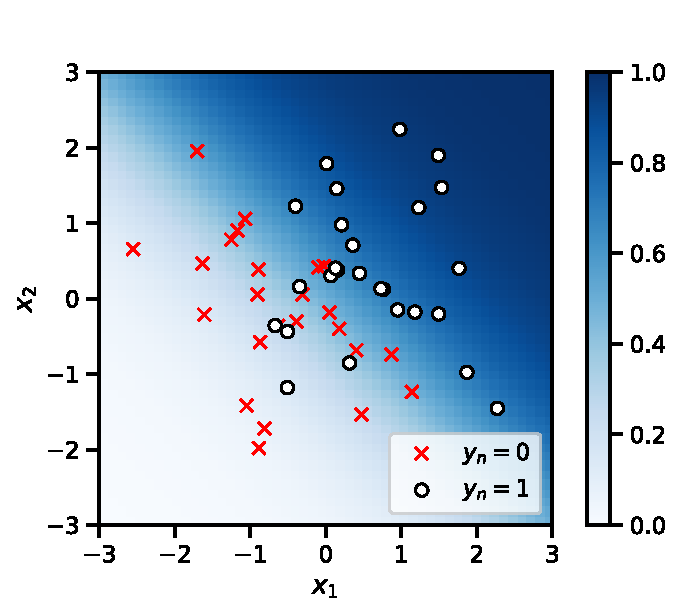
\includegraphics[width=1.\linewidth]{figures/lap2/data.pdf}
\end{column}

\end{columns}
\end{frame}

\begin{frame}{Logistic and probit functions}
Common choices for $f$ include the logistic and probit functions, corresponding to the \emph{logistic regression} and \emph{probit regression} models, respectively.

\centering
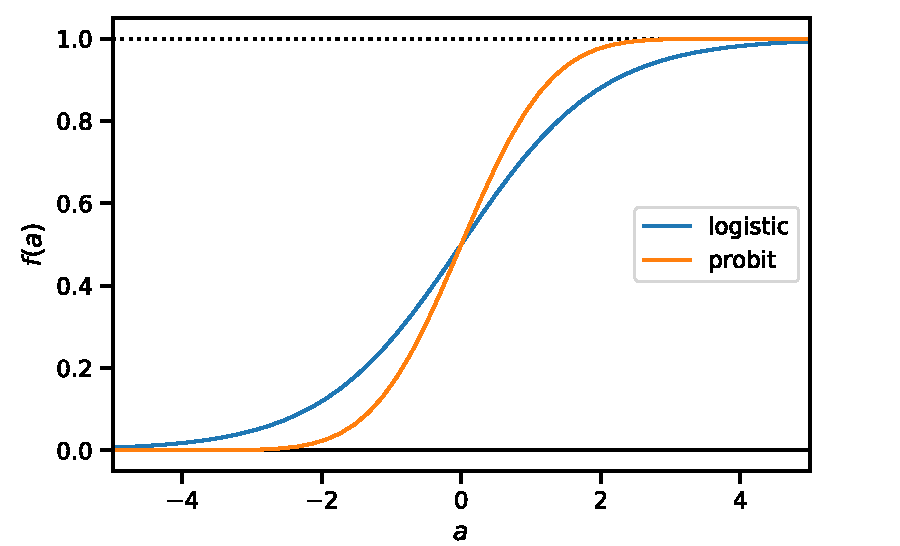
\includegraphics[width=.7\textwidth]{figures/lap2/logistic_probit.pdf}
\end{frame}

\begin{frame}{Likelihood}
The likelihood of $N$ conditionally independent observations is,
\begin{align}
    p(\{y_n\}_{n=1}^N \mid \{\mbx_n\}_{n=1}^N, \mbw) 
    &= 
    \prod_{n=1}^N \distBernoulli(y_n \mid f(\mbw^\top \mbx_n)) \\
    &= \prod_{n=1}^N f(\mbw^\top \mbx_n)^{y_n} \, (1-f(\mbw^\top \mbx_n))^{1-y_n}
\end{align}
For example, consider the \textit{logistic function} $f(a) = \frac{e^a}{1+e^{a}}$. Then,
\begin{align}
    p(\{y_n\}_{n=1}^N \mid \{\mbx_n\}_{n=1}^N, \mbw) 
    &= \prod_{n=1}^N \left[ \frac{e^{\mbw^\top \mbx_n}}{1+e^{\mbw^\top \mbx_n}} \right]^{y_n} 
    \left[ \frac{1}{1+e^{\mbw^\top \mbx_n}} \right]^{1-y_n}
    \\
    \label{eq:ch2_lkhd}
    &= \prod_{n=1}^N \frac{e^{\langle y_n \mbx_n, \, \mbw \rangle}}{1+e^{\mbw^\top \mbx_n}}
\end{align}

The numerator can be written in terms of $\sum_n y_n \mbx_n$, but the denominator doesn't easily simplify. 

\end{frame}


\begin{frame}{Prior}

\begin{itemize}

\item Here, we'll use a spherical multivariate normal prior,
\begin{align}
    p(\mbw) &= \cN(\mbw \mid \mbzero, \sigma^2 \mbI),
\end{align}
where $\mbzero \in \reals^P$ and $\sigma^2 \in \reals_+$ are the mean and variance, respectively.

\item This is the simplest choice, but we have lots of flexibility if a stronger prior is warranted.

\item For example, it's easy to generalize to arbitrary mean and covariance, $\mbmu$ and $\mbSigma$.

\end{itemize}

\end{frame}

\begin{frame}{Log probability contours}
    \centering
    \includegraphics[width=.75\textwidth]{figures/lap2/log_joint.pdf}
\end{frame}

\begin{frame}{Box's Loop: Infer hidden quantities}
\begin{center}
\includegraphics[width=.85\linewidth]{figures/lap1/boxsloop.jpeg}\\
\end{center} 
\begin{flushright}
{\footnotesize Blei, \textit{Ann. Rev. Stat. App.} 2014.}
\end{flushright}
\end{frame}

\begin{frame}{Box's Loop: Infer hidden quantities}
\begin{center}
\includegraphics[width=.85\linewidth]{figures/lap1/boxsloop.jpeg}\\
\end{center} 
\begin{flushright}
{\footnotesize Blei, \textit{Ann. Rev. Stat. App.} 2014.}
\end{flushright}
\end{frame}


\begin{frame}{Maximum a posteriori (MAP) estimation}

Before going to full Bayesian inference, let's just look for the posterior mode.

The log posterior probability is equal to the log joint minus the log marginal likelihood, which is constant with respect to the parameters $\mbw$,
\begin{align}
    \cL(\mbw) &= \log p(\{y_n\}_{n=1}^N \mid \{\mbx_n\}_{n=1}^N, \mbw) + \log p(\mbw) - \underbrace{\log p(\{y_n\}_{n=1}^N \mid \{\mbx_n\}_{n=1}^N)}_{\text{const. w.r.t. } \mbw} \\
    &= \sum_{n=1}^N \log \frac{e^{\langle y_n \mbx_n, \, \mbw \rangle}}{1+e^{\mbw^\top \mbx_n}} -\frac{1}{2\sigma^2} \mbw^\top \mbw + c\\
    &= \Big \langle \sum_{n=1}^N y_n \mbx_n, \mbw \Big \rangle 
    - \sum_{n=1}^N \log (1 + \exp \{\mbx_n^\top \mbw \}) - \frac{1}{2\sigma^2} \mbw^\top \mbw + c
\end{align}

\end{frame}

\begin{frame}{Gradient of the log probability}

Taking the gradient and setting it to zero,
\begin{align}
    \nabla_{\mbw} \cL(\mbw) &= 
    \sum_{n=1}^N y_n \mbx_n - \sum_{n=1}^N 
    \frac{\exp\{\mbx_n^\top \mbw\}}{1 + \exp \{\mbx_n^\top \mbw\}} \mbx_n
    - \frac{1}{\sigma^2} \mbw
    \\
    &= \sum_{n=1}^N y_n \mbx_n - \sum_{n=1}^N 
    f(\mbx_n^\top \mbw) \mbx_n.
    - \frac{1}{\sigma^2} \mbw
\end{align}
In matrix notation, 
\begin{align}
    \mbX = \begin{bmatrix} - & \mbx_1^\top & - \\ & \vdots & \\ - & \mbx_N^\top & - \end{bmatrix}, \quad \text{and} \quad  &
    \mby = \begin{bmatrix} y_1 \\ \vdots \\ y_N \end{bmatrix},
\end{align}
and letting $\hat{\mby} = f(\mbX \mbw)$, where $f$ is applied elementwise, we can write the gradient as,
\begin{align}
    \nabla_{\mbw} \cL(\mbw) &= (\mby - \hat{\mby})^\top \mbX - \frac{1}{\sigma^2} \mbw.
\end{align}
\end{frame}

\begin{frame}{Gradient of the log probability II}
\begin{itemize}
    \item In other words, the \textit{gradient of the log likelihood is a weighted sum of the covariates} where the weights are given by the error $y_n - \hat{y}_n$.
    
    \item Note that the gradient is still a \textit{nonlinear function of $\mbw$} since $\hat{y} = f(\mbx_n^\top \mbw)$. 
    
    \item The nonlinear equation $\nabla_{\mbw} \cL(\mbw) = 0$ does not have a closed form solution.
\end{itemize}


\end{frame}

\begin{frame}{Hessian of the log probability}

\begin{itemize}
\item The Hessian---i.e. the matrix of second partial derivatives, or the Jacobian of the gradient---is,
\begin{align}
    \nabla_{\mbw}^2 \cL(\mbw) &= 
    \nabla_{\mbw} \sum_{n=1}^N \Big(y_n - f(\mbx_n^\top \mbw) \Big) \mbx_n 
    - \frac{1}{\sigma^2} \mbw.
    \\
    &= -\left( \sum_{n=1}^N f'(\mbx_n^\top \mbw) \mbx_n \mbx_n^\top + \frac{1}{\sigma^2} \mbI \right)
\end{align}
where $f': \reals \to \reals$ is the derivative of $f$. 

\item Since $f$ is monotonically increasing, $f' \geq 0$.

\item The negative Hessian is a weighted sum of outer products with positive weights $f'(\mbx_n^\top \mbw)$. Thus, the Hessian is negative definite.

\item That means the \textit{log probability is concave} and has a global optimum.

\end{itemize}
\end{frame}

\begin{frame}{Concavity of the log probability}
    \centering
    \includegraphics[width=.75\textwidth]{figures/lap2/log_joint_1d.pdf}
\end{frame}


\begin{frame}[t]{Exercise: The derivative of the logistic function}

\textit{Show that}
\begin{align}
    f'(a) = \left[\frac{\dif}{\dif \alpha} \frac{e^\alpha}{1+e^\alpha}\right]_{\alpha=a} = f(a) (1 - f(a)) = f(a)f(-a) \geq 0.
\end{align}

\end{frame}


\begin{frame}{Algorithm}
\begin{itemize}

\item Though the MAP estimate doesn't have a closed form solution, we can find it via optimization. 

\item Since the log probability is concave, standard optimization methods will find the global optimum. 

\item For example, (damped) \emph{Newton's method},
\begin{align}
    \mbw^{(i+1)} &\leftarrow \mbw^{(i)} - \gamma [\nabla^2_{\mbw} \cL(\mbw^{(i)})]^{-1} \nabla_{\mbw} \cL(\mbw^{(i)}) 
\end{align}
(with sufficiently small step size $\gamma \in (0, 1]$) achieves second-order convergence to the optimum,~$\mbw_{\mathsf{MAP}}$.

\item With many covariates (when $P$ is large), Newton's method incurs an $O(P^3)$ complexity. 

\item \emph{Quasi}-Newton methods, like the BFGS algorithm, build an approximation to approximate Newton's method at lower computational cost. 

\end{itemize}

\end{frame}

\begin{frame}{BFGS Convergence}
    \centering
    \includegraphics[width=.75\textwidth]{figures/lap2/bfgs.pdf}
\end{frame}


\begin{frame}{Posterior Distribution}
What if we want more than a point estimate? 

The posterior distribution is given by,
\begin{align}
    p(\mbw \mid \{\mbx_n, y_n\}_{n=1}^N) &= \frac{p(\mbw) \, p(\{y_n\}_{n=1}^N \mid \mbw, \{\mbx_n\}_{n=1}^N)}{p(\{y_n\}_{n=1}^N \mid \{\mbx_n\}_{n=1}^N)} \\
\end{align}

Unfortunately, the marginal likelihood is hard to compute since 
\begin{align}
    p(\{y_n\}_{n=1}^N \mid \{\mbx_n\}_{n=1}^N) &=
    \int \prod_{n=1}^N \mathrm{Bern}(y_n \mid f(\mbw^\top \mbx_n)) \, \mathcal{N}(\mbw \mid 0, \sigma^2 \mbI) \dif \mbw
\end{align}
does not have a closed form solution.

\end{frame}

\begin{frame}{Laplace Approximation}

\textbf{Idea: } \textit{approximate the posterior with a multivariate normal distribution centered on the mode.}

To motivate this, consider a second-order Taylor approximation to the log posterior,
\begin{align}
    \cL(\mbw) &\approx \cL(\mbw_{\mathsf{MAP}}) + (\mbw - \mbw_{\mathsf{MAP}})^\top \underbrace{\nabla_{\mbw} \cL(\mbw_{\mathsf{MAP}})}_{\mbzero \text{ at the mode}} + \frac{1}{2} (\mbw - \mbw_{\mathsf{MAP}})^\top \nabla^2_{\mbw} \cL(\mbw_{\mathsf{MAP}}) (\mbw - \mbw_{\mathsf{MAP}}) \\
    &= -\frac{1}{2} (\mbw - \mbw_{\mathsf{MAP}})^\top \mbSigma \cL(\mbw_{\mathsf{MAP}}) (\mbw - \mbw_{\mathsf{MAP}}) + c \\
    &= \log \cN(\mbw \mid \mbw_{\mathsf{MAP}}, \mbSigma) 
\end{align}
where $\mbSigma = - [\nabla^2_{\mbw} \cL(\mbw_{\mathsf{MAP}})]^{-1} $

In other words, the posterior is approximately Gaussian with covariance given by the (negative) inverse Hessian at the mode.

Since the Hessian is \textit{negative} definite, the covariance is \emph{positive} definite, as required.
\end{frame}

\begin{frame}{Laplace Approximation II}
    
    \centering
    \includegraphics[width=.75\textwidth]{figures/lap2/laplace.pdf}
\end{frame}


\begin{frame}{Bernstein-von Mises Theorem}
    In the large data limit (as $N \to \infty$), the posterior is asymptotically normal, justifying the Laplace approximation in this regime.
    
    Consider a simpler setting in which we have data $\{y_n\}_{n=1}^N \iid{\sim} p(y \mid \theta_{\mathsf{true}})$.
    
    Under some conditions (e.g. $\theta_{\mathsf{true}}$ not on the boundary of $\Theta$ and $\theta_{\mathsf{true}}$ has nonzero prior probability), then the MAP estimate is consistent. As $N \to \infty$,  $\theta_{\mathsf{MAP}} \to \theta_{\mathsf{true}}$.
    
    Likewise,
    \begin{align} 
        p(\theta \mid \{y_n\}_{n=1}^N) \to \cN \big(\theta \mid \theta_{\mathsf{true}}, \tfrac{1}{N} [J(\theta_{\mathsf{true}})]^{-1} \big)
    \end{align}
    where 
    \begin{align}
        J(\theta) &= -\E_{p(y | \theta)} \left[ \frac{\dif^2}{\dif \theta^2} \log p(y \mid \theta) \right]
    \end{align}
    is the \emph{Fisher information} of parameter $\theta$.
\end{frame}

\begin{frame}{Approximating the marginal likelihood}

The Laplace approximation also offers an approximation of the intractable marginal likelihood,
\begin{align}
    \cL(\mbw_{\mathsf{MAP}}) &= 
    \log p(\mbw_{\mathsf{MAP}}) + \log p(\{y_n\}_{n=1}^N \mid \mbw_{\mathsf{MAP}}, \{\mbx_n\}_{n=1}^N) - \log p(\{y_n\}_{n=1}^N \mid \{\mbx_n\}_{n=1}^N) \\
    & \approx \log \cN(\mbw_{\mathsf{MAP}} \mid \mbw_{\mathsf{MAP}}, \mbSigma) \\
    &= -\frac{P}{2} \log (2 \pi) - \frac{1}{2} \log |\mbSigma|
\end{align}
Rearranging terms,
\begin{align}
    \nonumber
    \log p(\{y_n\}_{n=1}^N \mid \{\mbx_n\}_{n=1}^N) 
    &\approx \log p(\mbw_{\mathsf{MAP}}) + \log p(\{y_n\}_{n=1}^N \mid \mbw_{\mathsf{MAP}}, \{\mbx_n\}_{n=1}^N) \\
    &\qquad + \frac{P}{2} \log (2 \pi) + \frac{1}{2} \log |\mbSigma|
\end{align}

\textbf{Note:} combine this with $\mbSigma \approx \tfrac{1}{N} [J(\mbw_{MAP})]^{-1}$ and $\tfrac{1}{2} \log |\mbSigma| \approx \tfrac{P}{2} \log N + O(1)$ to derive the \emph{Bayesian information criterion (BIC)}, a technique for penalized maximum likelihood estimation.
\end{frame}

\begin{frame}{Exponential family distributions}
    
    Now we'll consider GLMs with \emph{exponential family} observations,
    \begin{align}
        p(y_n \mid \eta_n) &= h(y_n) \exp \left \{\langle t(y_n), \eta_n \rangle - A(\eta_n) \right\},
    \end{align}
    where 
    \begin{itemize}
        \item $h(y_n): \cY \to \reals_+$ is the \emph{base measure},
        \item $t(y_n) \in \reals^T$ are the \textit{sufficient statistics},
        \item $\eta_n \in \reals^T$ are the \textit{natural parameters}, and
        \item $A(\eta_n): \reals^T \to \reals$ is the \textit{log normalizing} function (aka the \emph{partition function}).
    \end{itemize}
    
\end{frame}

\begin{frame}{Example: Bernoulli distribution in exponential family form}
    The Bernoulli distribution is a special case, 
    \begin{align}
        \distBernoulli(y_n \mid p_n) &= p_n^{y_n} \, (1-p_n)^{1 - y_n} \\
        &= \exp \left\{ y_n \log p_n + (1-y_n) \log (1- p_n) \right \} \\
        &= \exp \left\{ y_n \log \frac{p_n}{1 - p_n} + \log (1 - p_n) \right \}  \\
        &= h(y_n) \exp \left\{ y_n \eta_n - A(\eta_n) \right \} 
    \end{align}
    where
    \begin{align}
        h(y_n) &= 1 & 
        t(y_n) &= y_n & 
        \eta_n &= \log \frac{p_n}{1- p_n} &
        A(\eta_n) &= -\log ( 1 - p_n) \\
        & & & & & & &= - \log \left(1 - \frac{e^{\eta_n}}{1 + e^{\eta_n}} \right) \\
        % & & & & & & &= - \log \frac{1}{1 + e^{\eta_n}}  \\
        & & & & & & &= \log \left(1 + e^{\eta_n} \right).
    \end{align}
\end{frame}

\begin{frame}{Gradient of the log normalizer yields the expected sufficient statistics}
    
    By definition,
    \begin{align}
        A(\eta_n) &= \log \int h(y_n) \exp \left \{\langle t(y_n), \eta_n \rangle \right\} \dif y_n
    \end{align}
    so
    \begin{align}
        \nabla_{\eta_n} A(\eta_n) 
        &= \nabla_{\eta_n} \log \int h(y_n) \exp \left \{\langle t(y_n), \eta_n \rangle \right\} \dif y_n \\
        &= \frac{\int h(y_n) \exp \left \{\langle t(y_n), \eta_n \rangle \right\} t(y_n) \dif y_n}{\int h(y_n) \exp \left \{\langle t(y_n), \eta_n \rangle \right\} \dif y_n} \\
        &= \int p(y_n \mid \eta_n) \, t(y_n) \dif y_n \\
        &= \E_{p(y_n | \eta_n)}[t(y_n)]
    \end{align}
    
\end{frame}

\begin{frame}{Hessian of the log normalizer yields the covariance of the sufficient statistics}
    
    Likewise,
    \begin{align}
        \nabla^2_{\eta_n} A(\eta_n) 
        &= \nabla_{\eta_n} \int p(y_n \mid \eta_n) \, t(y_n) \dif y_n \\
        &= \int p(y_n \mid \eta_n) \, t(y_n) \, (t(y_n) - \nabla_{\eta_n} A(\eta_n))^\top \dif y_n \\
        &= \E_{p(y_n | \eta_n)}[t(y_n) t(y_n)^\top ] - \E_{p(y_n | \eta_n)}[t(y_n)] \, \E_{p(y_n | \eta_n)}[t(y_n)]^\top \\
        &= \mathrm{Cov}_{p(y_n | \eta_n)}[t(y_n)]
    \end{align}
    
    Covariances are positive semi-definite, so the \textit{log normalizer is a convex function}.
\end{frame}

\begin{frame}{Exponential family GLMs}
    \begin{itemize}
        \item To construct a generalized linear model with exponential family observations, we set 
    \begin{align}
        \E[y_n \mid \mbx_n] &= f(\mbw^\top \mbx_n).
    \end{align}
    
    \item From above, this implies,
    \begin{align}
        \nabla_{\eta_n} A(\eta_n) &= f(\mbw^\top \mbx_n) \\
        \Rightarrow \eta_n &= [\nabla A]^{-1} \big( f(\mbw^\top \mbx_n) \big),
    \end{align}
    when $\nabla A(\cdot)$ is invertible. (In this case, the exponential family is said to be \emph{minimal}).
    
    \item The \emph{canonical mean function} is $f(\cdot) = \nabla A(\cdot)$ so that $\eta_n = \mbw^\top \mbx_n$.
    
    \item The (canonical) \emph{link function} is the inverse of the (canonical) mean function.
    \end{itemize}
    
\end{frame}

\begin{frame}{Logistic regression revisited}
    Consider the Bernoulli distribution once more. The gradient of the log normalizer is,
    \begin{align}
        \nabla_\eta A(\eta) &= \nabla_\eta \log (1 + e^\eta) 
        = \frac{e^\eta}{1+ e^\eta}
    \end{align}
    This is the logistic function!
    
    Thus, logistic regression with is a Bernoulli GLM with the canonical mean function.
\end{frame}

\begin{frame}{Why care about canonical mean functions?}

(\textbf{Spoiler:} It's 2021 and we have automatic differentiation so it's not such a big deal anymore.)

Canonical mean functions lead to nice math. Consider the log joint probability,
\begin{align}
    \cL(\mbw) &= \log p(\mbw) + \sum_{n=1}^N \langle t(y_n), \eta_n \rangle - A(\eta_n)  + c \\
    &= -\frac{1}{2\sigma^2} \mbw^\top \mbw + \sum_{n=1}^N \langle t(y_n), \mbw^\top \mbx_n \rangle - A(\mbw^\top \mbx_n) + c,
\end{align}
where we have assumed $p(\mbw) = \cN(\mbw \mid \mbzero, \sigma^2 \mbI)$ and canonical mean function so $\eta_n = \mbw^\top \mbx_n$.

The gradient is,
\begin{align}
    \nabla_{\mbw} \cL(\mbw) 
    &= -\frac{1}{\sigma^2}\mbw + \sum_{n=1}^N \langle t(y_n), \mbx_n \rangle - \langle \nabla A(\mbw^\top \mbx_n), \, \mbx_n \rangle\\
    &= -\frac{1}{\sigma^2}\mbw + \sum_{n=1}^N \langle t(y_n) - \E_{p(y_n | \mbw^\top \mbx_n)}[t(y_n)], \, \mbx_n \rangle
\end{align}

\end{frame}

\begin{frame}{Why care about canonical mean functions? II}

In many cases, $t(y_n) = y_n \in \reals$ so
\begin{align}
    \nabla_{\mbw} \cL(\mbw) 
    &= -\frac{1}{\sigma^2}\mbw + \sum_{n=1}^N (y_n - \hat{y}_n) \mbx_n.
\end{align}

And in that case the Hessian is
\begin{align}
    \nabla^2_{\mbw} \cL(\mbw) 
    &= -\frac{1}{\sigma^2}\mbI - \sum_{n=1}^N \nabla^2 A(\mbw^\top \mbx_n) \, \mbx_n \mbx_n^\top \\
    &= -\left( \frac{1}{\sigma^2}\mbI + \sum_{n=1}^N \mathrm{Var}_{p(y_n | \mbw^\top \mbx_n)}[y_n] \, \mbx_n \mbx_n^\top \right)
\end{align}

\end{frame}

\begin{frame}{Why care about canonical mean functions? III}

Now recall the Newton's method updates, written here in terms of the change in weights,
\begin{align}
    \Delta \mbw &= - [\nabla_{\mbw}^2 \cL(\mbw)]^{-1} \nabla_{\mbw} \cL(\mbw) \\
    &= \left[\frac{1}{\sigma^2}\mbI + \sum_{n=1}^N \mathrm{Var}_{p(y_n | \mbw^\top \mbx_n)}[y_n] \, \mbx_n \mbx_n^\top \right]^{-1} \left[ -\frac{1}{\sigma^2}\mbw + \sum_{n=1}^N (y_n - \hat{y}_n) \mbx_n \right]
\end{align}

Letting $\hat{v}_n = \mathrm{Var}_{p(y_n | \mbw^\top \mbx_n)}[y_n]$ and taking the uninformative limit of $\sigma^2 \to \infty$, 
\begin{align}
    \Delta \mbw &=
    \left[\sum_{n=1}^N \hat{v}_n \, \mbx_n \mbx_n^\top \right]^{-1} \left[ \sum_{n=1}^N (y_n - \hat{y}_n) \mbx_n \right] \\
    % &= (\mbX^\top \hat{\mbV} \mbX)^{-1} [\mbX^\top \hat{\mbV} \hat{\mbV}^{-1} (\mby - \hat{\mby})] \\
    &= (\mbX^\top \hat{\mbV} \mbX)^{-1} [\mbX^\top \hat{\mbV} \hat{\mbz}]
\end{align}
where $\hat{\mbV} = \diag([\hat{v}_1, \ldots, \hat{v}_N])$ and $\hat{\mbz} = \hat{\mbV}^{-1} (\mby - \hat{\mby})$. 

This is \emph{iteratively reweighted least squares} (IRLS) with weights $\hat{v}_n$ and targets $\hat{z}_n = \frac{y_n - \hat{y}_n}{\hat{v}_n}$, both of which are functions of the current weights $\mbw$.
\end{frame}

\begin{frame}{Next time: Posterior predictive checks}
\begin{center}
\includegraphics[width=.85\linewidth]{figures/lap1/boxsloop.jpeg}\\
\end{center} 
\begin{flushright}
{\footnotesize Blei, \textit{Ann. Rev. Stat. App.} 2014.}
\end{flushright}
\end{frame}


\end{document}
